In order for robots to become widely accessible, users must be able to command them by specifying high-level behaviors, rather than programming low-level robot controllers.
This type of robot control has recently become possible by applying tools and ideas from formal methods and hybrid systems to the field of robotics. The resulting methodologies translate high-level tasks to discrete and subsequently low-level continuous controllers in a correct-by-construction manner \cite{BBEFKP06, KGFP_TRO09, KaramanCDC2009, Wongpiromsarn2010, LaValleRSS2011, BhatiaRAM2011, Belta2013RSS}.
%\emph{Reactive} approaches account for a dynamic -- and possibly adversarial -- environment, and are thus of particular interest. For example, the framework in \cite{KGFP_TRO09} takes a logic formula that contains the mission specification and, by solving a two-player game between the robot and its environment \cite{piterman_06}, outputs a hybrid controller that is guaranteed to accomplish the mission. Other reactive approaches have been proposed, e.g., in \cite{Wongpiromsarn2010} and \cite{Belta2013RSS}.
\emph{Reactive} approaches, e.g. \cite{KGFP_TRO09, Wongpiromsarn2010, Belta2013RSS}, account for a dynamic -- and possibly adversarial -- environment, and are thus of particular interest.

These approaches operate under the closed-world assumption. The robot only accounts for what was modeled before execution, and no information can be added autonomously, i.e. without a human re-specifying the mission.
% Ref: http://c2.com/cgi/wiki?ClosedWorldAssumption
However, robots have moved from the cloistered assembly line to such highly unstructured workspaces as the Fukushima Daiichi nuclear disaster site \cite{Fukushima2011}. 
%Thus, there is a need for high-level robot controllers that adapt to the discrepancies between the robot's model of the world and reality. 
In addition, robots are sometimes asked to incorporate new functions during execution. 
Examples include 
%reconfigurable modular robots \cite{ModularIROS2011}, as well as 
robots that learn on-the-fly \cite{SaxenaIJRR2012} or query online knowledge repositories \cite{rapyuta2013}. 
Finally, the world may be open with respect to goals added after the robot has been deployed, as in the case of urban search and rescue tasks \cite{MatthiasAI2010}, military scenarios \cite{gda2013}, and autonomous space and planetary exploration missions \cite{spaceXplore2006}. 

\begin{myExample}\label{Ex:mailbot1}
Consider a robotic courier, i.e., a ``mailbot", (see Fig. \ref{Fig:mailbot}) deployed in a school or company building. 
Its task is to collect letters and deliver them to the recipients' offices. 
This mission is relatively simple, and yet the robot's world is already open w.r.t. letters addressed to recipients about which the robot does not know. % Na to kana entelws nia-nia dew?
%Even if all possible recipients, and the locations of their offices, are fixed, the information may not be available a priori.
\end{myExample}

%\begin{figure}[t]
%	\centering
%	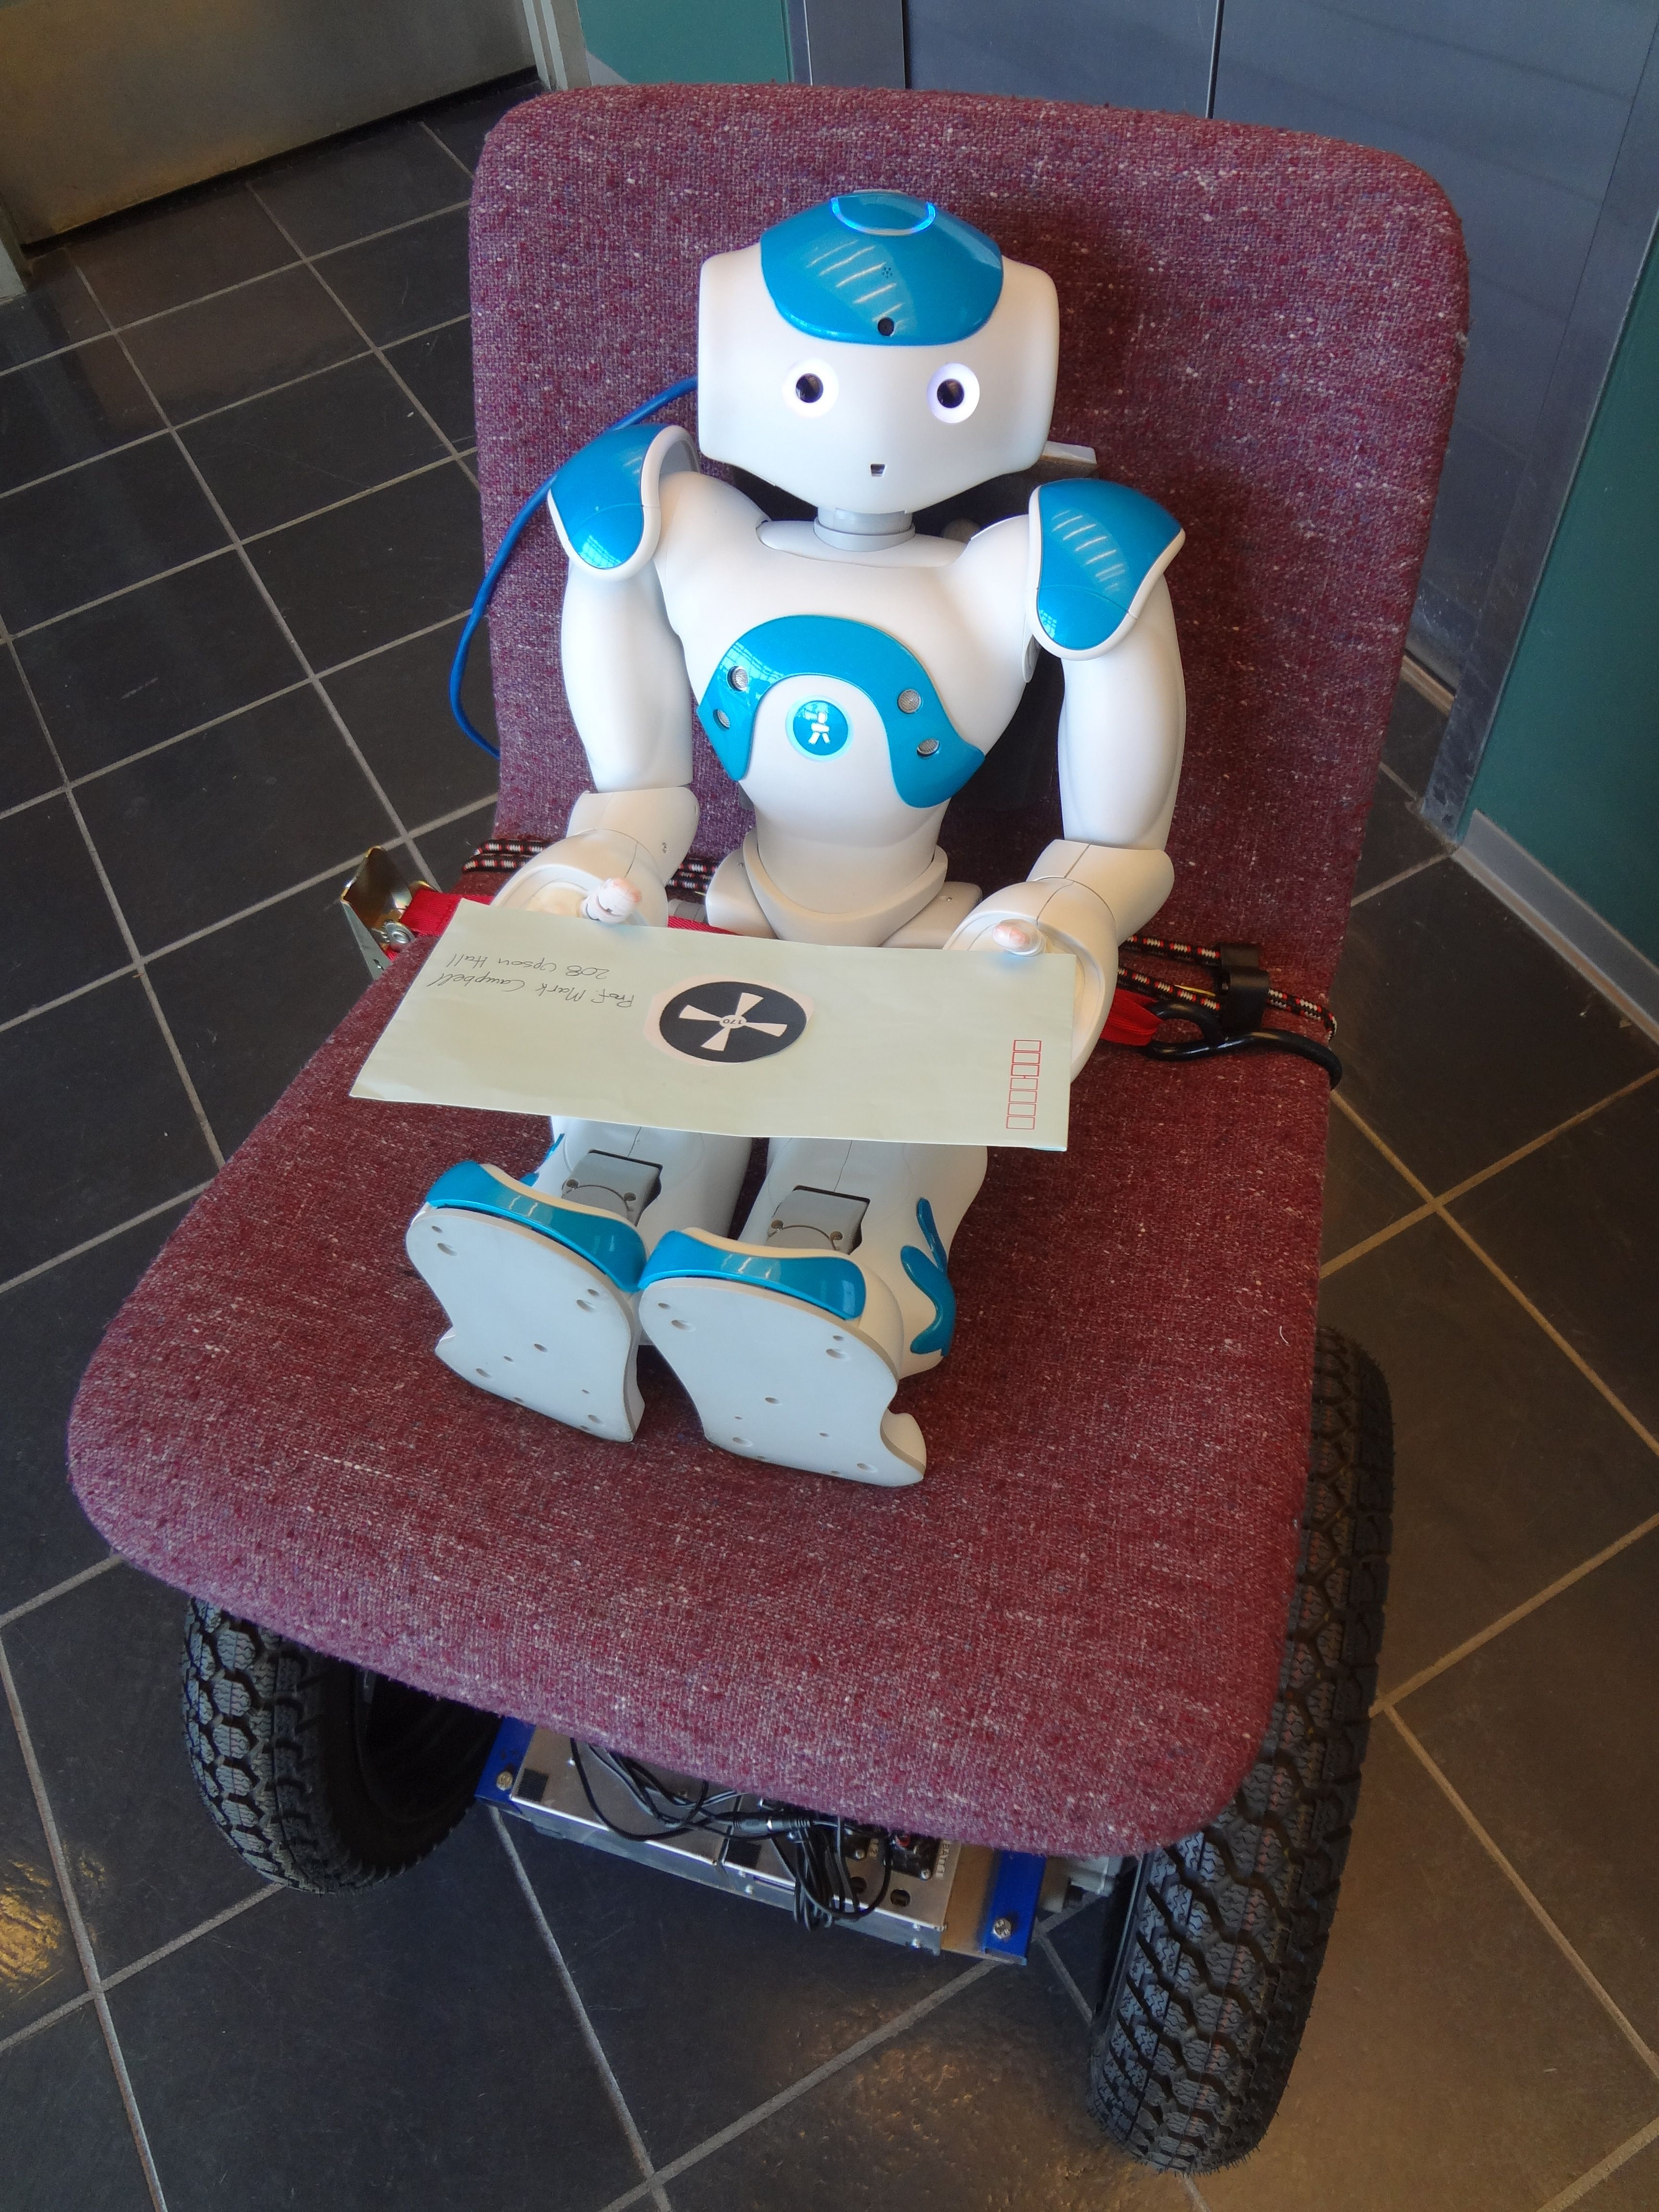
\includegraphics[width=0.7\columnwidth, clip]{./img/mailbot.jpg}
%	\caption{Above is our implementation of a mailbot. An Aldebaran Nao humanoid robot is mounted on a Segway platform that includes a Lidar sensor. The actuation and perception capabilities of the Nao are complemented by the localization, navigation and mobility advantages of the Segway.}
%	\label{Fig:mailbot}
%\end{figure}

\begin{figure}[t]
	\centering
	
	\begin{subfigure}[b]{0.493\columnwidth}
	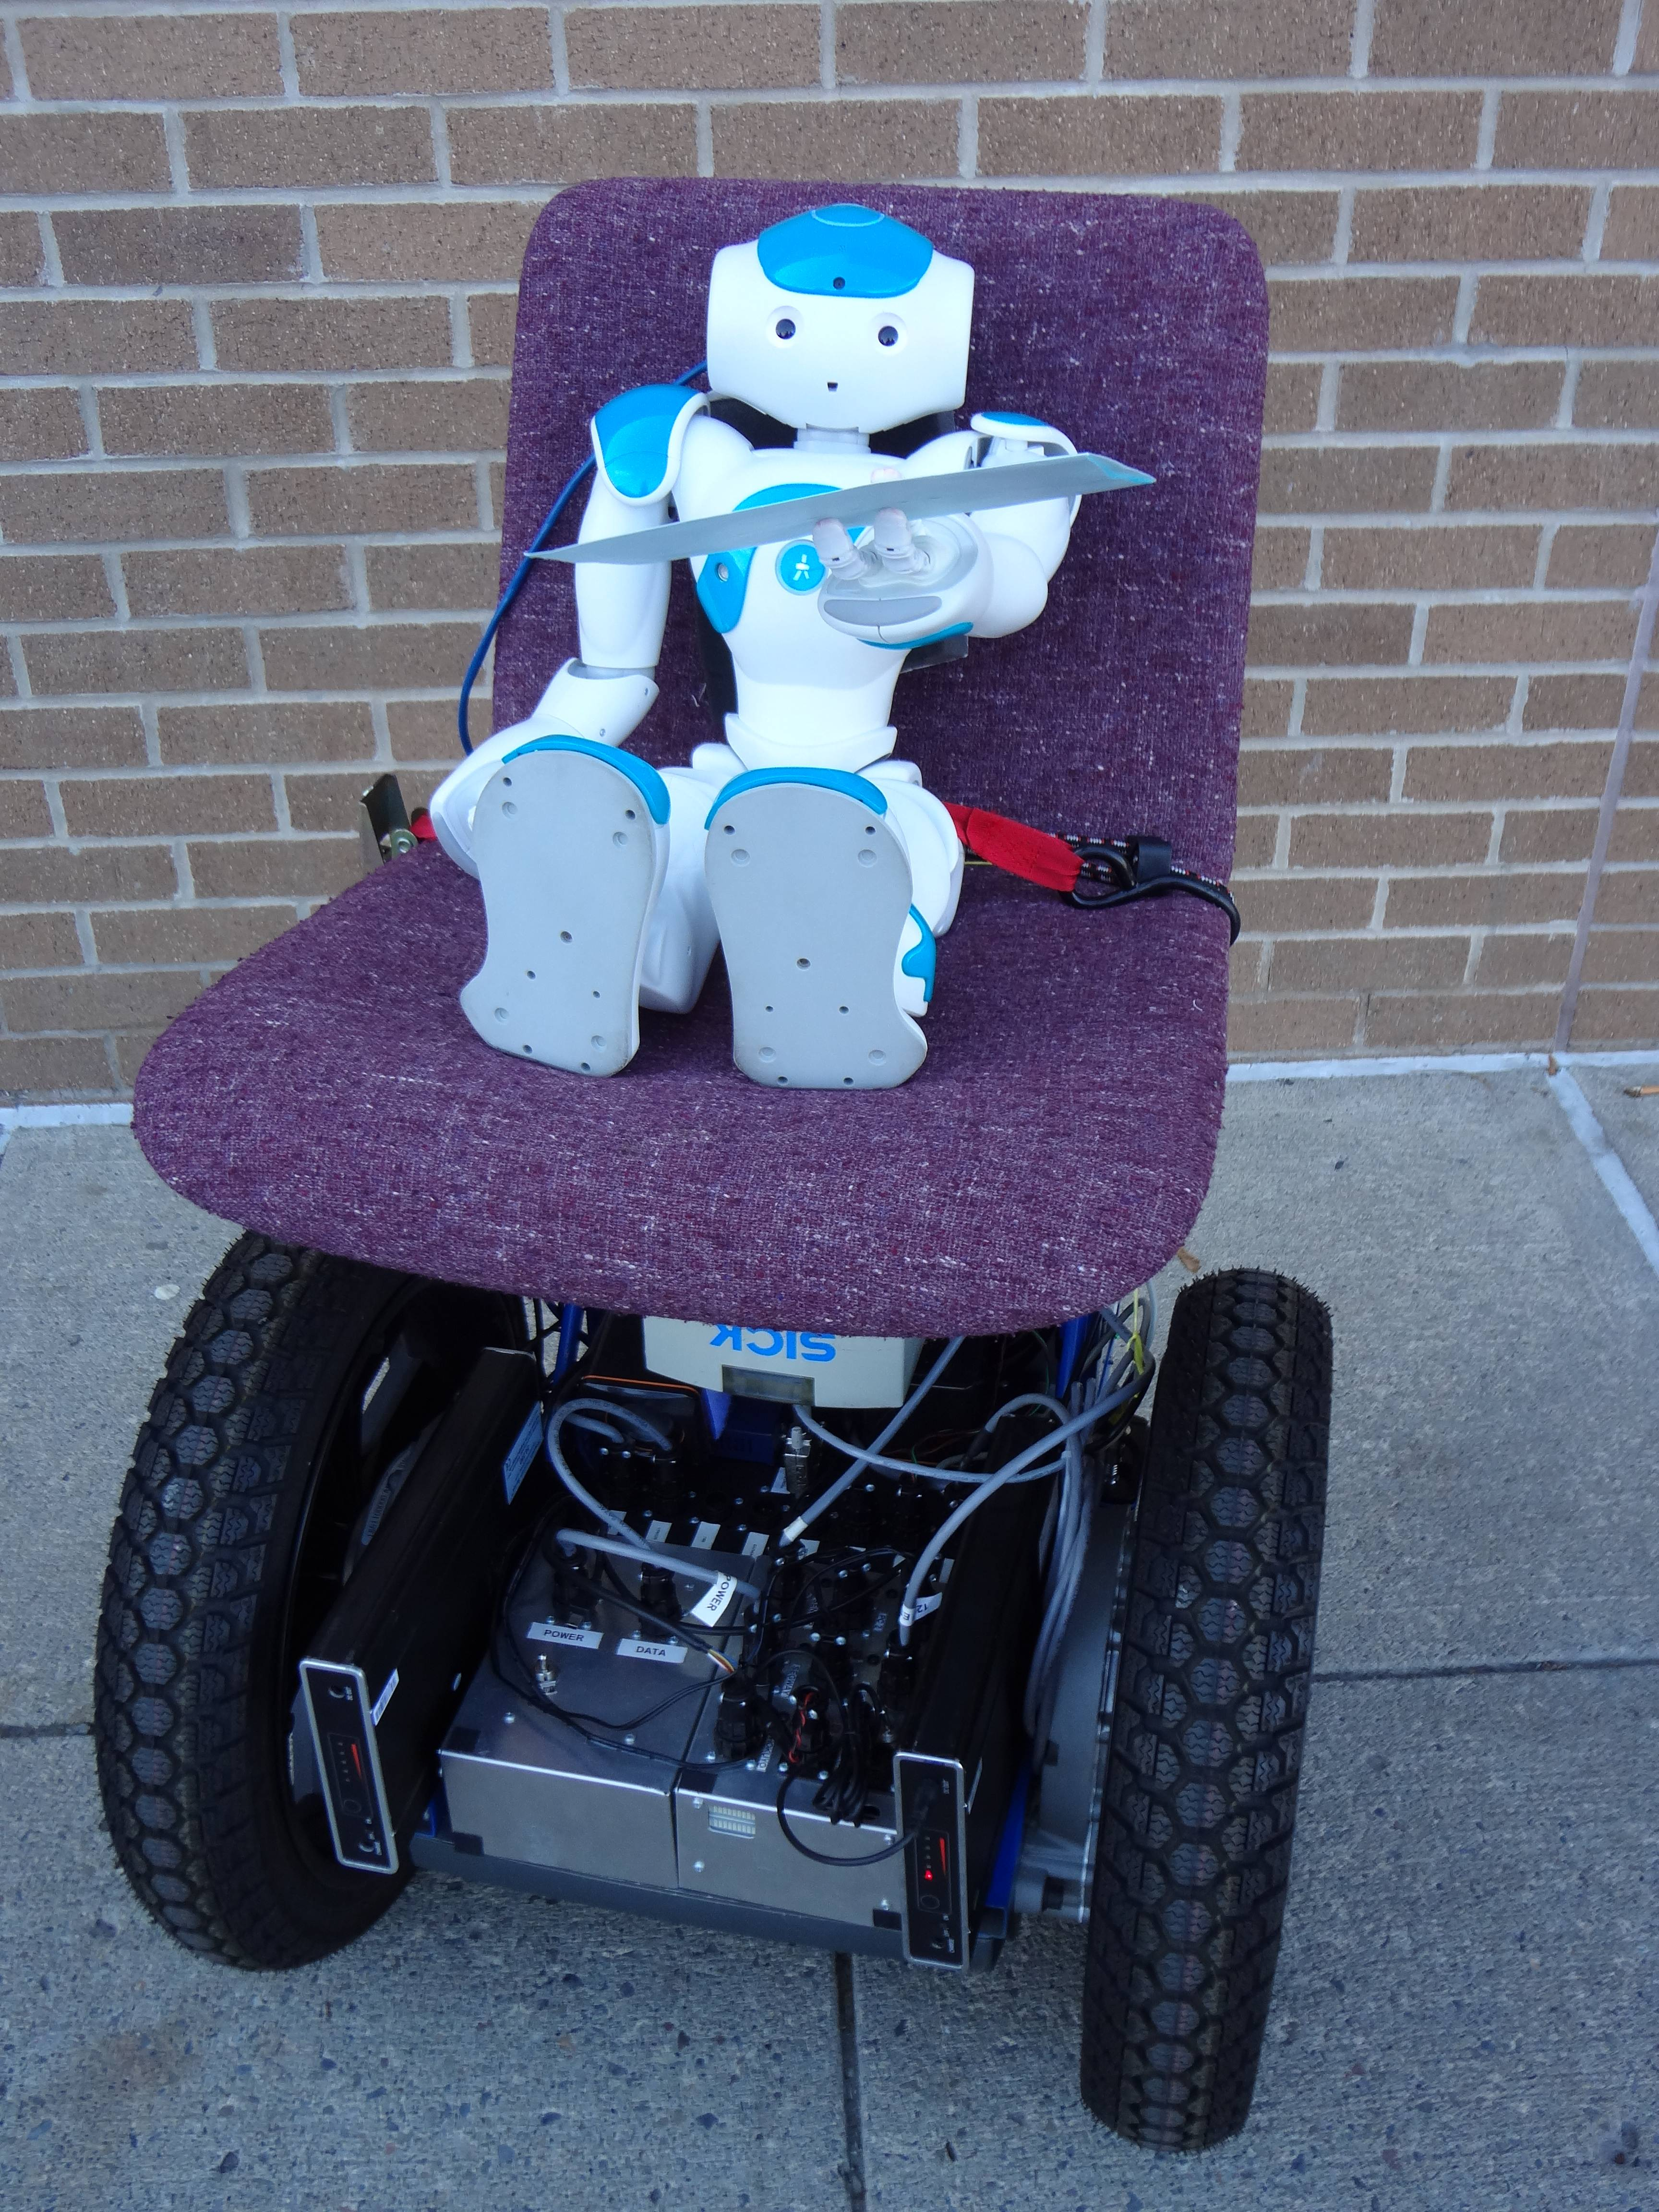
\includegraphics[width=\columnwidth]{img/mailbot_front.jpg}
	\end{subfigure}
	\hfill
	\begin{subfigure}[b]{0.493\columnwidth}
	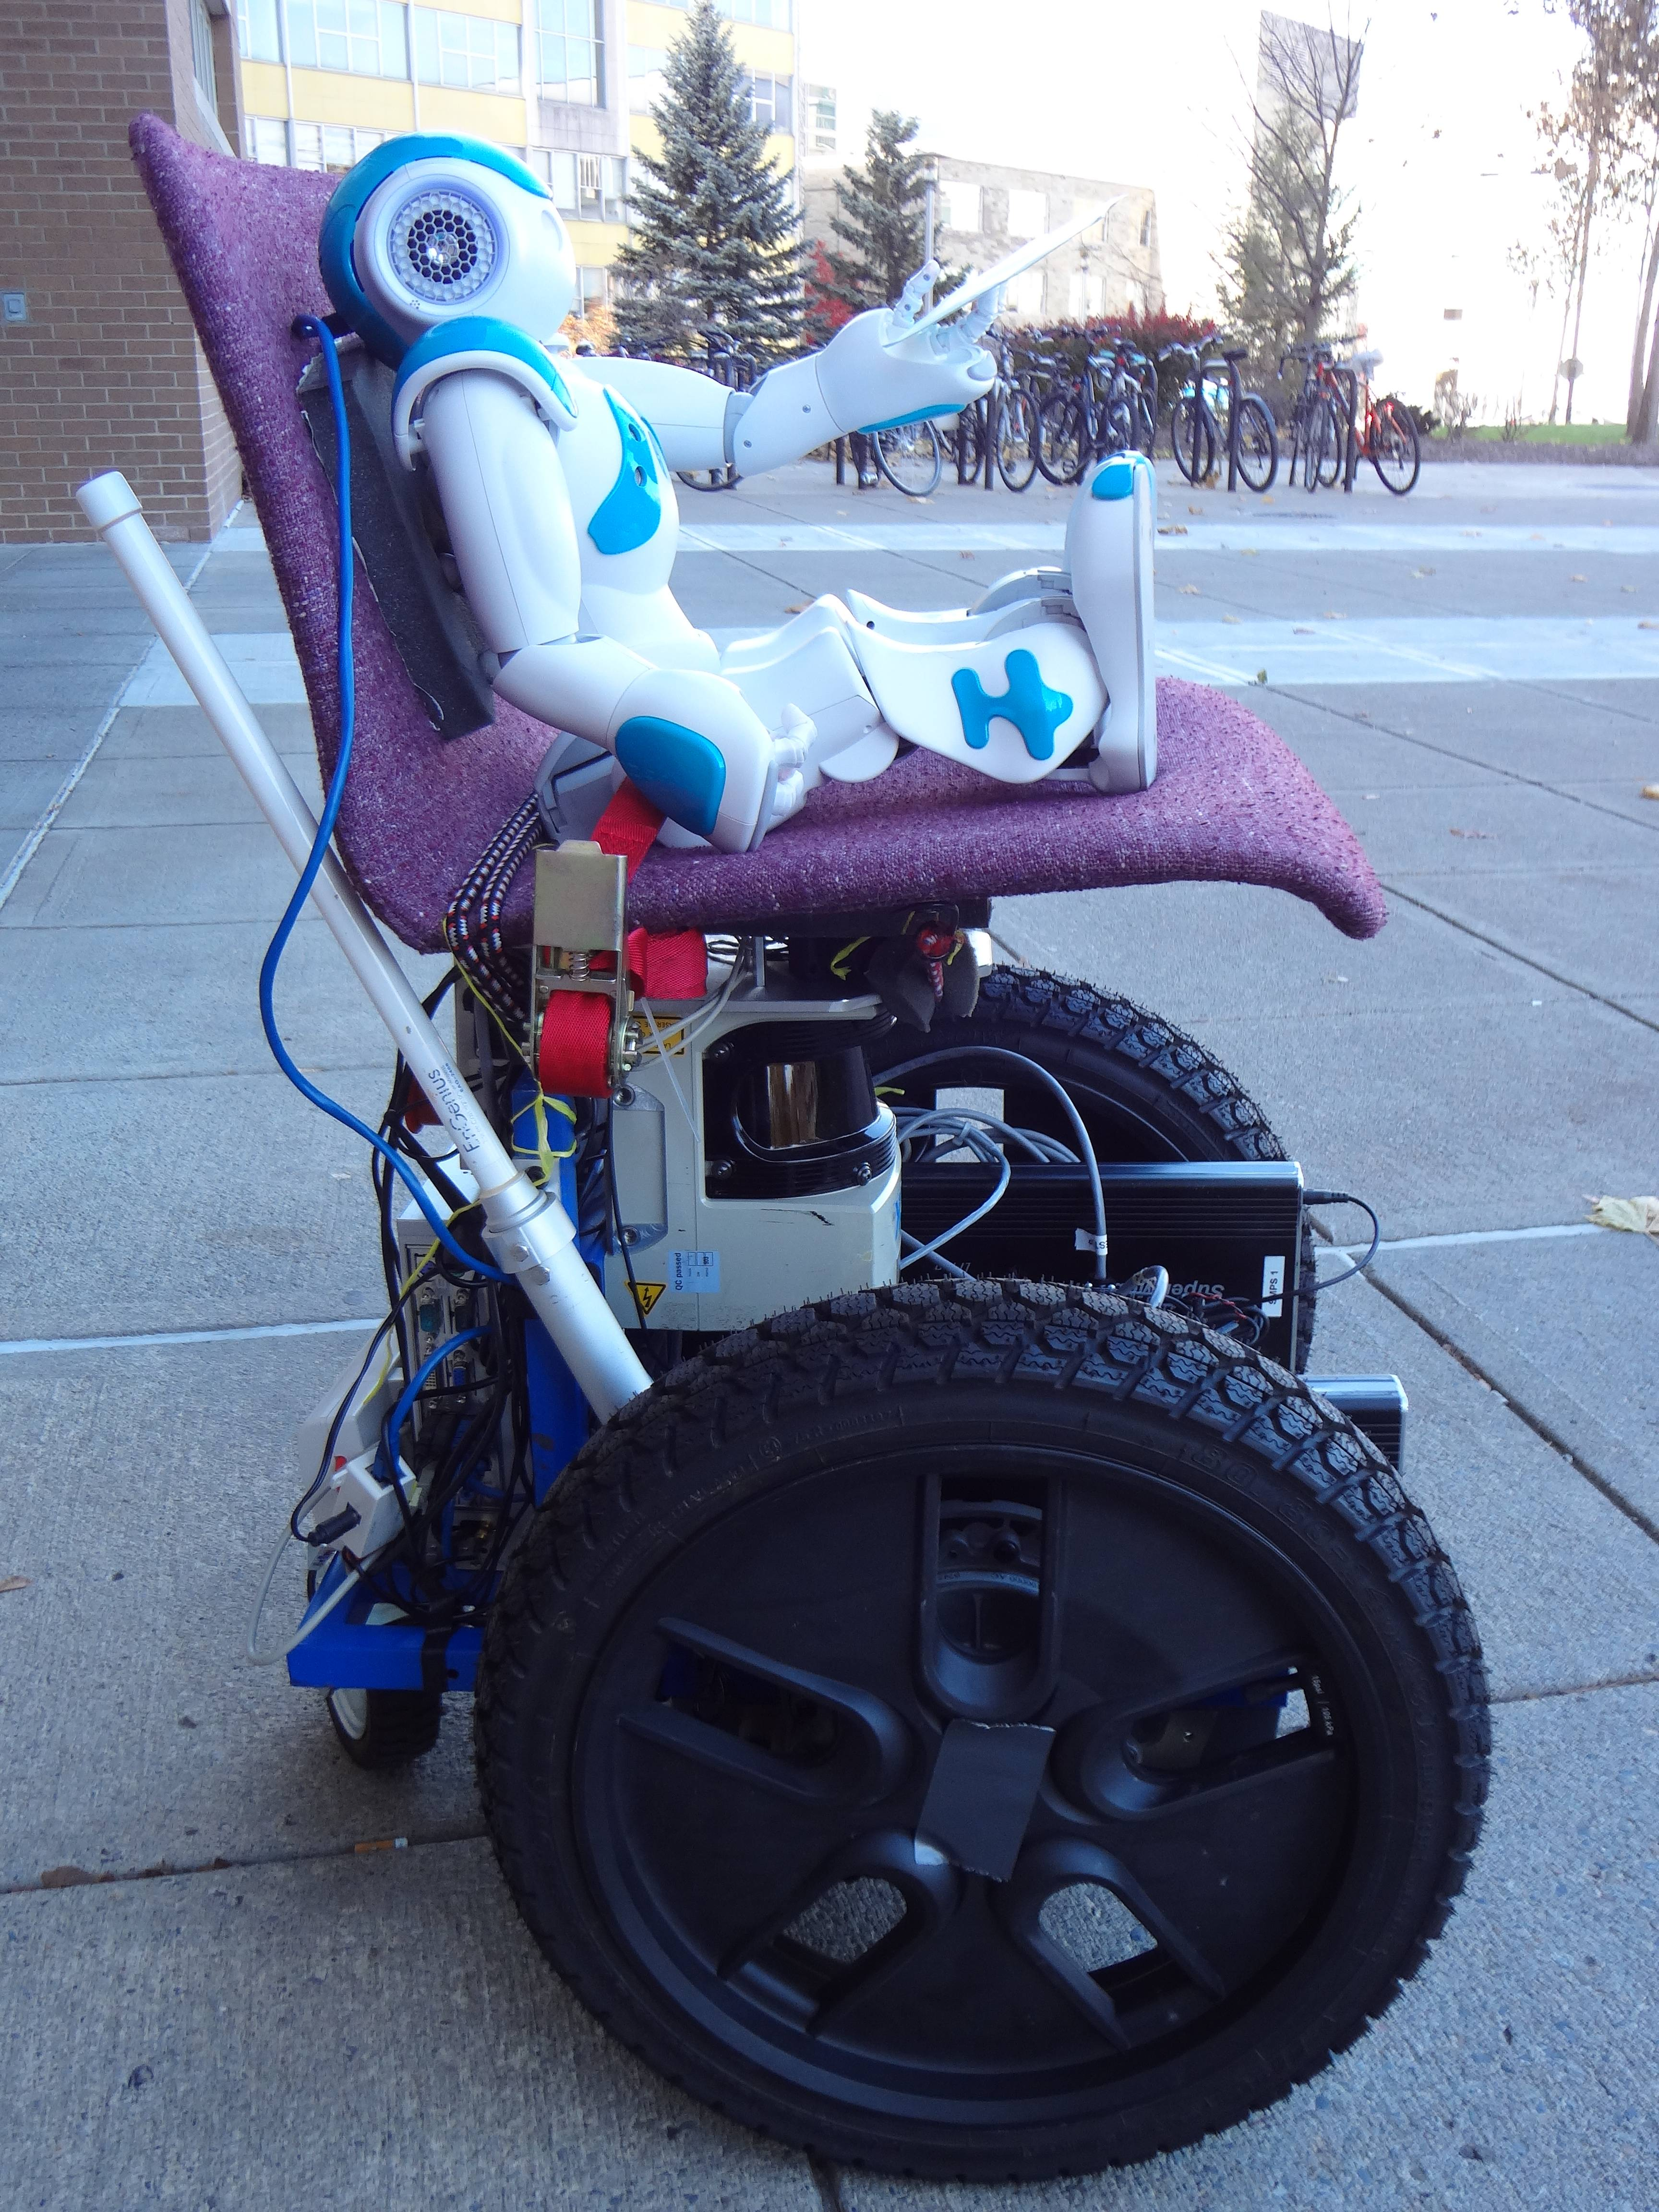
\includegraphics[width=\columnwidth]{img/mailbot_side.jpg}
	\end{subfigure}	
	\caption{Our robotic courier: an Aldebaran Nao humanoid robot is mounted on a Segway-based, mobility and sensing platform.}
	\label{Fig:mailbot}
	\vspace{-5 pt}
\end{figure}

In order to obtain controllers for open worlds, a number of challenges have to be overcome. 
First, the world can be open w.r.t. its spatial components. An aspect of this issue has been tackled in \cite{MurrayICRA2012} and \cite{MurrayICRA2013a}, where the authors introduced local resynthesis as a way to account for local topological changes in the robot's workspace. 
Additionally, an approach that addresses the unreactive equivalent of the same problem appeared in \cite{Dimos2013ICRA}. 
Furthermore, the aforementioned approaches deal with changes in the internal structure of the workspace. We are interested in expanding the workspace upon discovery of new regions.
In addition, we are interested in augmenting the mission with additional objectives, a situation that may arise if the robot can discover new regions or objects of interest. 
The work in \cite{BingxinRSS2012} allows the robot's workspace to expand, but does not account for the discovery of non-spatial aspects of the world, such as learning new actions or responding to unexpected events.
Moreover, there is the the challenge of specifying open-world missions in the first place, since the world is only partially known prior to execution. 
Specification languages and abstractions have been developed for similar tasks with both formal \cite{Joshi2012, MatthiasAI2010} and statistical \cite{Tellex2011} methods.
This paper differs from previous approaches in its use of correct-by-construction controller synthesis in an open world, requiring new techniques.

%In this paper, we first propose an approach to writing high-level missions such that the robot's tasks can be specified in terms of elements in the world that are unknown prior to execution. This is accomplished via \emph{open-world abstractions}, which allow us to specify behaviors implicitly. 
In this paper, we first propose \emph{open-world abstractions}, which allow us to specify high-level robot behaviors in terms of elements in the world that are unknown prior to execution.
Furthermore, they allow the specification to be updated in an autonomous fashion, as new elements of interest are discovered. The new elements include, but are not limited to, the sensing of new objects and events, and the discovery of new regions of the workspace, and they may lead to new mission constraints and/or goals.
We show how the mission specification can be systematically and automatically rewritten on-the-fly, in order to correctly incorporate these new elements of the open world. 
%Finally, our high-level approach allows the user to control how the new elements will be accounted for, and when the updated specification should be translated to a new controller.
Finally, our high-level approach allows the user to control how the new elements will be accounted for, and when the robot should start operating according to the updated mission specification. Therefore, our work differs from, and is complementary to, \cite{MurrayICRA2012} and \cite{MurrayICRA2013a}, which focus on directly revising the robot's discrete controller to account for changes in the workspace.

The paper is organized as follows: Section \ref{preliminaries} provides the necessary background on logic-based reactive mission planning. Section \ref{problem} formally states the problem we are addressing. The proposed abstractions, which we will use to specify tasks over open worlds, are defined in Section \ref{abstractions}. Section \ref{openworld} presents our approach to systematically rewriting the mission specification. Simulations of the mailbot scenario (Example \ref{Ex:mailbot1}), which is revisited throughout the paper, are provided in Section \ref{simulation}. Finally, our conclusions, as well as possible research directions, are summarized in Section \ref{conclusion}.

% END